\documentclass[tikz,border=4pt]{standalone}
\usepackage{amsmath,amssymb}
\usetikzlibrary{arrows.meta,positioning,calc}

\begin{document}
\begin{tikzpicture}[
  >={Stealth[length=2mm]},
  img/.style={draw, line width=0.5pt, inner sep=0pt},
  lab/.style={font=\scriptsize, inner sep=1pt, align=center},
  hdr/.style={font=\small\bfseries, black!80},
  ar/.style={->, line width=0.6pt, black!85},
]

\node[img] (full) at (0,0) {
\includegraphics[width=3.1cm]{sym_full.png}};
\node[lab, below=2pt of full] {$G\in\{0,1\}^{64\times64}$\\occupied $0.399$};

\node[img] (q) at (5.3,0) {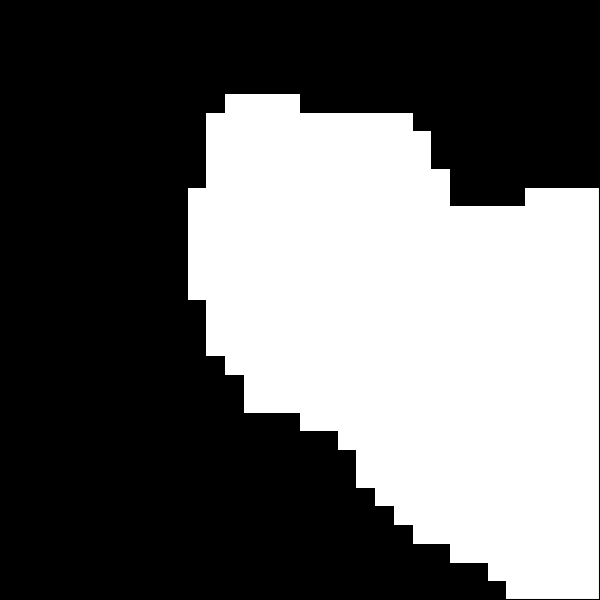
\includegraphics[width=1.55cm]{sym_quad.png}};
\node[lab, below=2pt of q] {$Q\in\{0,1\}^{32\times32}$\\one quarter of the cell};

\node[img] (r) at (10.6,0) {
\includegraphics[width=3.1cm]{sym_rebuild.png}};
\node[lab, below=2pt of r] {$\hat G\in\{0,1\}^{64\times64}$\\$\hat G = G$ exactly};

\draw[ar] (full.east) -- node[above, lab, yshift=1pt] {take\\quadrant} (q.west);
\draw[ar] (q.east) -- node[above, lab, yshift=1pt] {fliplr,\\flipud} (r.west);

\node[hdr] at (0,1.85) {(a) held-out sample};
\node[hdr] at (5.3,1.15) {(b) predicted quadrant};
\node[hdr] at (10.6,1.85) {(c) reflected design};

\end{tikzpicture}
\end{document}
